\documentclass[]{article}
 
\begin{document}
\section{Klassen per module}
Hierin worden alle grote klassen beschreven per module die gebruikt worden in de IDE. Elke klasse wordt kort toegelicht over hun functie, welke ADT's gebruikt hebben alsook hoe alle klassen samenwerken.

\subsection{Exceptions}
De verantwoordelijkheden van deze module worden beschreven in Sectie \ref{ExceptionsModule}.
\subsubsection{TypeException}
Deze wordt opgeroepen als er op runtime een type error gebeurt. De uitvoer van het uitvoerend proces wordt dan gestopt. De andere blijven doorgaan.
\subsubsection{ProcesFinishedException}
Deze exception wordt opgeroepen als een proces geen blocks meer bevat om uit te voeren.
\subsubsection{LockedException}
Deze Exception wordt opgeroepen als er een member variable van een Instance wordt aangesproken die gelocked is.
\subsubsection{OutOfBoundsException}
Deze exception wordt opgeroepen in CharAtBlock als in foute index wordt meegegeven.

\clearpage
 \begin{sidewaysfigure}
  \centering
   
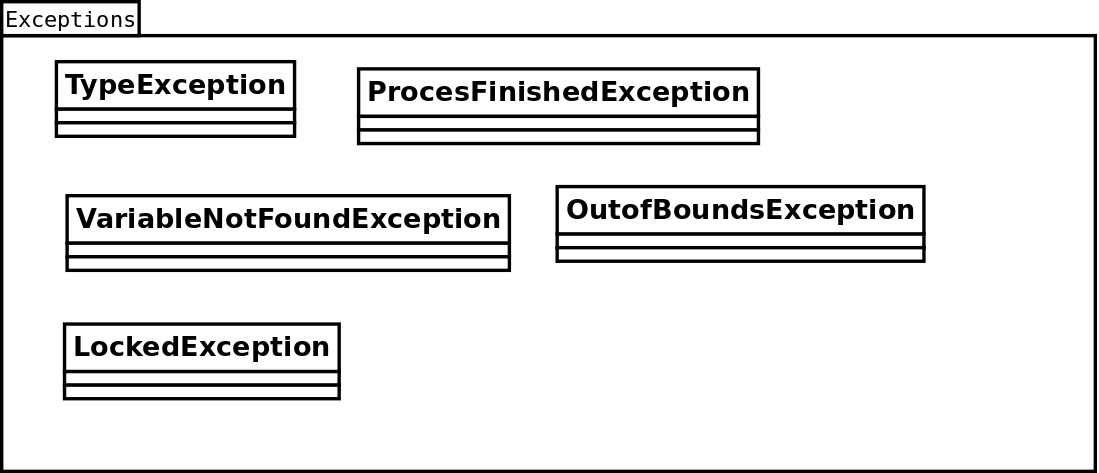
\includegraphics[scale=0.8]{./AnalyseClassenDiagram/exceptions.png}
  \caption{Exceptions Module.} \label{exceptionUML}
\end{sidewaysfigure}
\clearpage

\subsection{Variables}
De verantwoordelijkheden van deze module worden beschreven in Sectie \ref{VariablesModule}.
\subsubsection{EventInstance}
Een event bevat een Event voor zijn type Event waarvan het een instance is bij te houden en een Hashmap \cite{hashmap} waarbij het de naam van een variable (String) mapt op een variabele.
\subsubsection{ReturnVariables}
De ReturnVariables is klasse die gebruikt om return values in op te slaan en terug aan de functioncall. Deze bevat een stack \cite{stack} waarop de return waarde worden geduwt. Op deze manier kunnen we meerdere return values mogelijk maken. Echter voorzien we eerst maar een return value.
\subsubsection{Type}
\label{Type}
Dit is Enumeratie die een van de volgende kan zijn: Boolean, String, Number, Event of Value. Een value is een letterlijke inputwaarde door de gebruiker. Deze is nog niet geconverteerd naar een feitelijk type en kan dus eenderwelk type voorstellen.
\subsubsection{Abstact Class Variable}
\label{variable}
Deze klasse stelt een variabele voor. Deze heeft een Type als member.
\subsubsection{BooleanVariable}
Deze wordt afgeleid van de Abstact Class Variable en bevat dus een boolean als variable.
\subsubsection{NumberVariable}
Deze wordt afgeleid van de Abstact Class Variable en bevat dus een number als variable.
\subsubsection{StringVariable}
Deze wordt afgeleid van de Abstact Class Variable en bevat dus een String als variable.

\clearpage
 \begin{sidewaysfigure}
  \centering
   
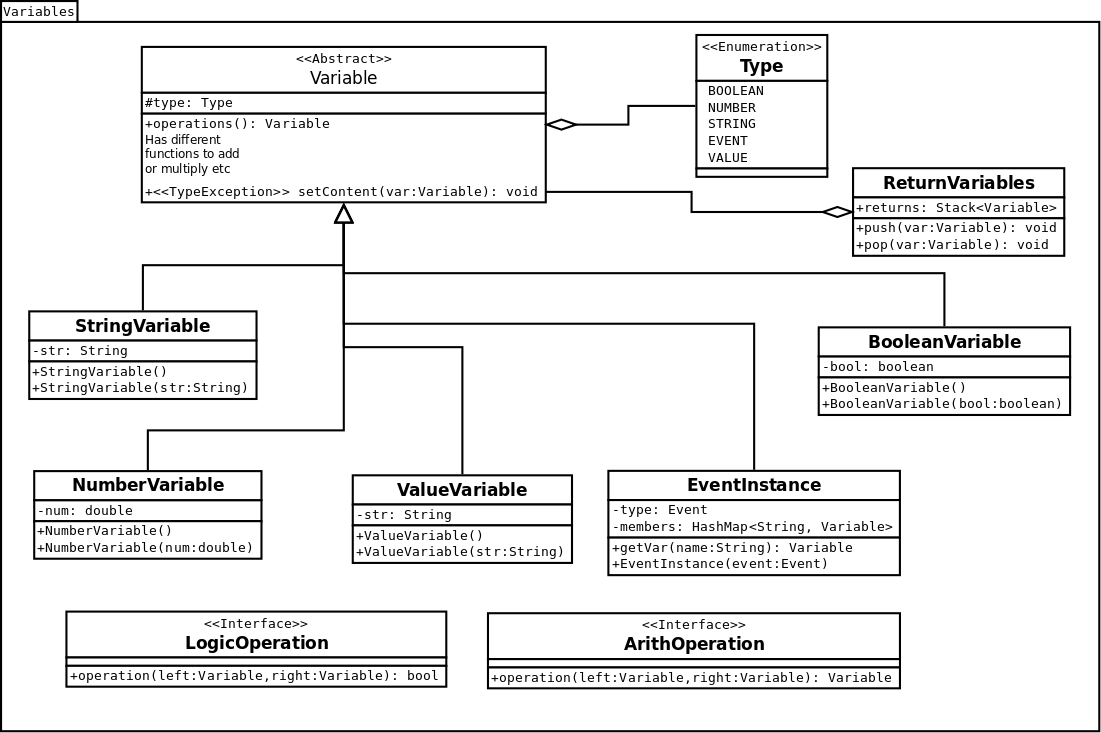
\includegraphics[scale=0.8]{./AnalyseClassenDiagram/variables.png}
  \caption{Variables Module.}
\end{sidewaysfigure}
\clearpage

\subsection{Blocks}
De verantwoordelijkheden van deze module worden beschreven in Sectie \ref{BlocksModule}.
\subsubsection{De Interface Block}
Een Block stelt een klasse voor die een bepaald stuk code voorstelt. Deze bevat een execute functie die een proces meekrijgt zodat hij zijn code kan uitvoeren of plaaten op het proces.
\subsubsection{HandlerBlock}
Deze implementeert de interface Block. Deze bevat een \texttt{ArrayList<Block>} \cite{arraylist} die we de body noemen. De heeft een EventInstance die hij mee kreeg op oproep, via zijn constructor. Deze wordt mee op zijn variabele stack gepushed bij het aanmaken van zijn FunctionFrame. De execute van deze block pushed de body als individuele blokken op de stack van het proces dat hij meekrijgt. Achteraan de body plakt hij nog een PopBlock.
\subsubsection{PopBlock}
Deze implementeert de interface Block. De execute van deze Block popt het bovenste FunctionFrame van de stack van het proces.
\subsubsection{AccessBlock}
 Deze bevat twee Strings namelijk de naam van het EventInstance waarvan het een member wil opvragen. En de naam van die member. De execute functie zal dus het EventInstance van de FunctionFrame opvragen. Hierin vraagt hij de variable op van de member en deze geeft hij terug.
\subsubsection{BroadCastBlock}
Bevat een naam van het Event. En een Hashmap \cite{hashmap} van Strings die de members van het event voorstellen deze worden gemapt op Blocks. De execute van dit Block zal deze Blocks uitvoeren en de bekomen variabele kopieren en mappen op de juiste string. Het zal dan een aangemaakte event terug geven aan het proces. Dat dit op zijn beurt doorgeeft aan de VM.
\subsubsection{FunctionBlock}
Deze implementeert de interface Block. Deze bevat een \texttt{ArrayList<Block>} \cite{arraylist} die we de body noemen. De excute functie van deze Block zet de body op Stack van Blocks van het proces dat deze meekrijgt. Onder deze body plakt hij nog PopBlock. De Block bevat twee \texttt{ArrayList<VariableBlock>} \cite{arraylist} voor respectievelijke parameters en return parameters.
\subsubsection{FunctionCallBlock}
Deze bevat een String voor de functie naam. En twee \texttt{ArrayList<String>} \cite{arraylist} voor respectievelijk de parameters en return waardes van de Call.\\ De execute van deze Block zal de variabele van de waarde parameters ophalen uit het huidige bovenste FunctieFrame van de Stack van het proces. Deze slaat hij tijdelijk lokaal op. Hierna haalt hij de namen van de parameters van de functie op. Hij maakt een nieuwe FunctieFrame hierop pushed hij alle parametersnamen met de eerder opgehaalde variabelen. Hierna pushed hij op Stack de SetBlocken voor de return waardes. Uiteindelijk roept hij de execute van de functie aan zodat deze bovenaan de stack staat. Dit telt als een primitieve stap.
\subsubsection{ReturnBlock}
Deze block bevat een \texttt{ArrayList} \cite{arraylist} van Strings die de namen van de variables voorstellen die gereturned moeten worden. Deze zal hij ophalen in het huidige FunctieFrame en opslaan in de ReturnVariables van het proces. Een ReturnBlock popt alle blokken van de Stack tot hij een PopBock tegenkomt.
\subsubsection{VariableBlock}
Deze Block bevat een String en een Type. De execute van deze block zal deze variable aanmaken en op het huidige FunctionFrame zetten.

\subsubsection{SetBlock}
Deze bevat een String die de naam is van een variabele op de huidige FunctionFrame. Deze block bevat nog een andere block, dat ofwel een variable, value of operatie aanduid. De execute van eender van deze blocken geeft steeds de inhoud (variable) terug aan de SetBlock. Deze blok telt als een primitieve stap.
\subsubsection{ArithBlock}
Deze block bevat een left block en een right block. Als deze twee worden geexecute op de teruggeven variable wordt de juiste operatie uitgevoerd de bekomen variabele wordt terug gegeven. De block bevat ook een statische hashmap zoals beschreven in sectie \ref{lambda} om de juiste operatie uit te kunnen voeren.
De uitvoering zal dus in een primitieve stap gebeuren.
\subsubsection{Random}
De execute van deze block geeft een random value tussen een lower- en upperBound terug in een Variabele. De lower- en upperBound kunnen weer blokken zijn die worden execute en een variabele teruggeven.
\subsubsection{ConcatBlock}
De execute van deze block geeft een variable terug die de string concatinatie van de een left- en rightBlock is. Deze Blocken kunnen dieper genest zijn maar hun execute geeft een variable terug.
\subsubsection{StrlenBlock}
Deze block geeft een variable terug die de lengte van de String bevat. Het bevat een Block die op zijn execute een Stringvariable terug geeft.
\subsubsection{CharAtBlock} 
Deze block geeft een variable terug die een string op een gegeven index. De String wordt meegeven als een block en deze geeft dus een variabele terug. De block die de string bevat kan dus genest zijn. Als die index niet gevonden is, dan wordt er een OutOfBoundsException gegooid.
\subsubsection{LogicBlock}
De execute van deze block geeft een variable terug. Deze block bevat een left block en een right block. Als deze twee worden geexecute op de teruggeven variable wordt de juiste operatie uitgevoerd de bekomen variabele wordt terug gegeven.
De uitvoering zal dus in een primitieve stap gebeuren. De block bevat ook een statische hashmap zoals beschreven in sectie \ref{lambda} om de juiste operatie uit te kunnen voeren.
\subsubsection{LockBlock}
Deze block lockt een bepaalde membervariabele van de instance waarbij het huidige proces hoort.
\subsubsection{UnlockBlock}
Deze block unlockt een bepaalde membervariabele van de instance waarbij het huidige proces hoort.
\subsubsection{ForeverBlock}
Deze block bevat een \texttt{ArrayList<Block>} \cite{arraylist} die we body noemen. De execute van deze block zet al zijn blokken op de stack met onderaan de body ook nog eens zichzelf geplakt.
\subsubsection{WhileBlock}
Deze bevat een Block conditie en een \texttt{ArrayList<Block>} \cite{arraylist} die we body noemen. De execute van de block kijkt als de conditie naar true evalueert door deze te laten execute en de waarde van de variable na te kijken. Zo ja dan wordt de body plus zichzelf op de stack van het proces gepushed.
\subsubsection{IfElseBlock}
Deze block bevat een Block conditie en twee \texttt{ArrayList<Block>} \cite{arraylist} die respecitievelijk de body van de If en else voorstellen. De execute van de block kijkt als de conditie naar true evalueert door deze te laten execute en de waarde van de variable na te kijken. Zo ja dan wordt de body van de If  op de stack van het proces gepushed anders de body van de Else.
\subsubsection{HideBlock}
Voert een functie van de instance uit om te hiden.
\subsubsection{ShowBlock}
Voert een functie van de instance uit om te showen.
\subsubsection{ChangeAppereanceBlock}
De bevat een Block index, deze kan een arith expression zijn. Dus we laten hem execute zodat we de index krijgen in een variable. Dit zal de execute van de blok doen plus het oproepen van de functie bij een instance die de appereance veranderd.
\subsubsection{MoveBlock}
Deze bevat een x- en een y-Block. De execute van de MoveBlock zal de waarde van x en y bekomen door deze Blocks te execute. De waardes geeft hij mee aan een functie van de instance die zijn x en y verhoogt met die waardes.
\subsubsection{PrintBlock}
Deze bevat een Block die geexecute wordt en de waarde van de variable wordt uitgeprint.


\clearpage
 \begin{sidewaysfigure}
  \centering
   
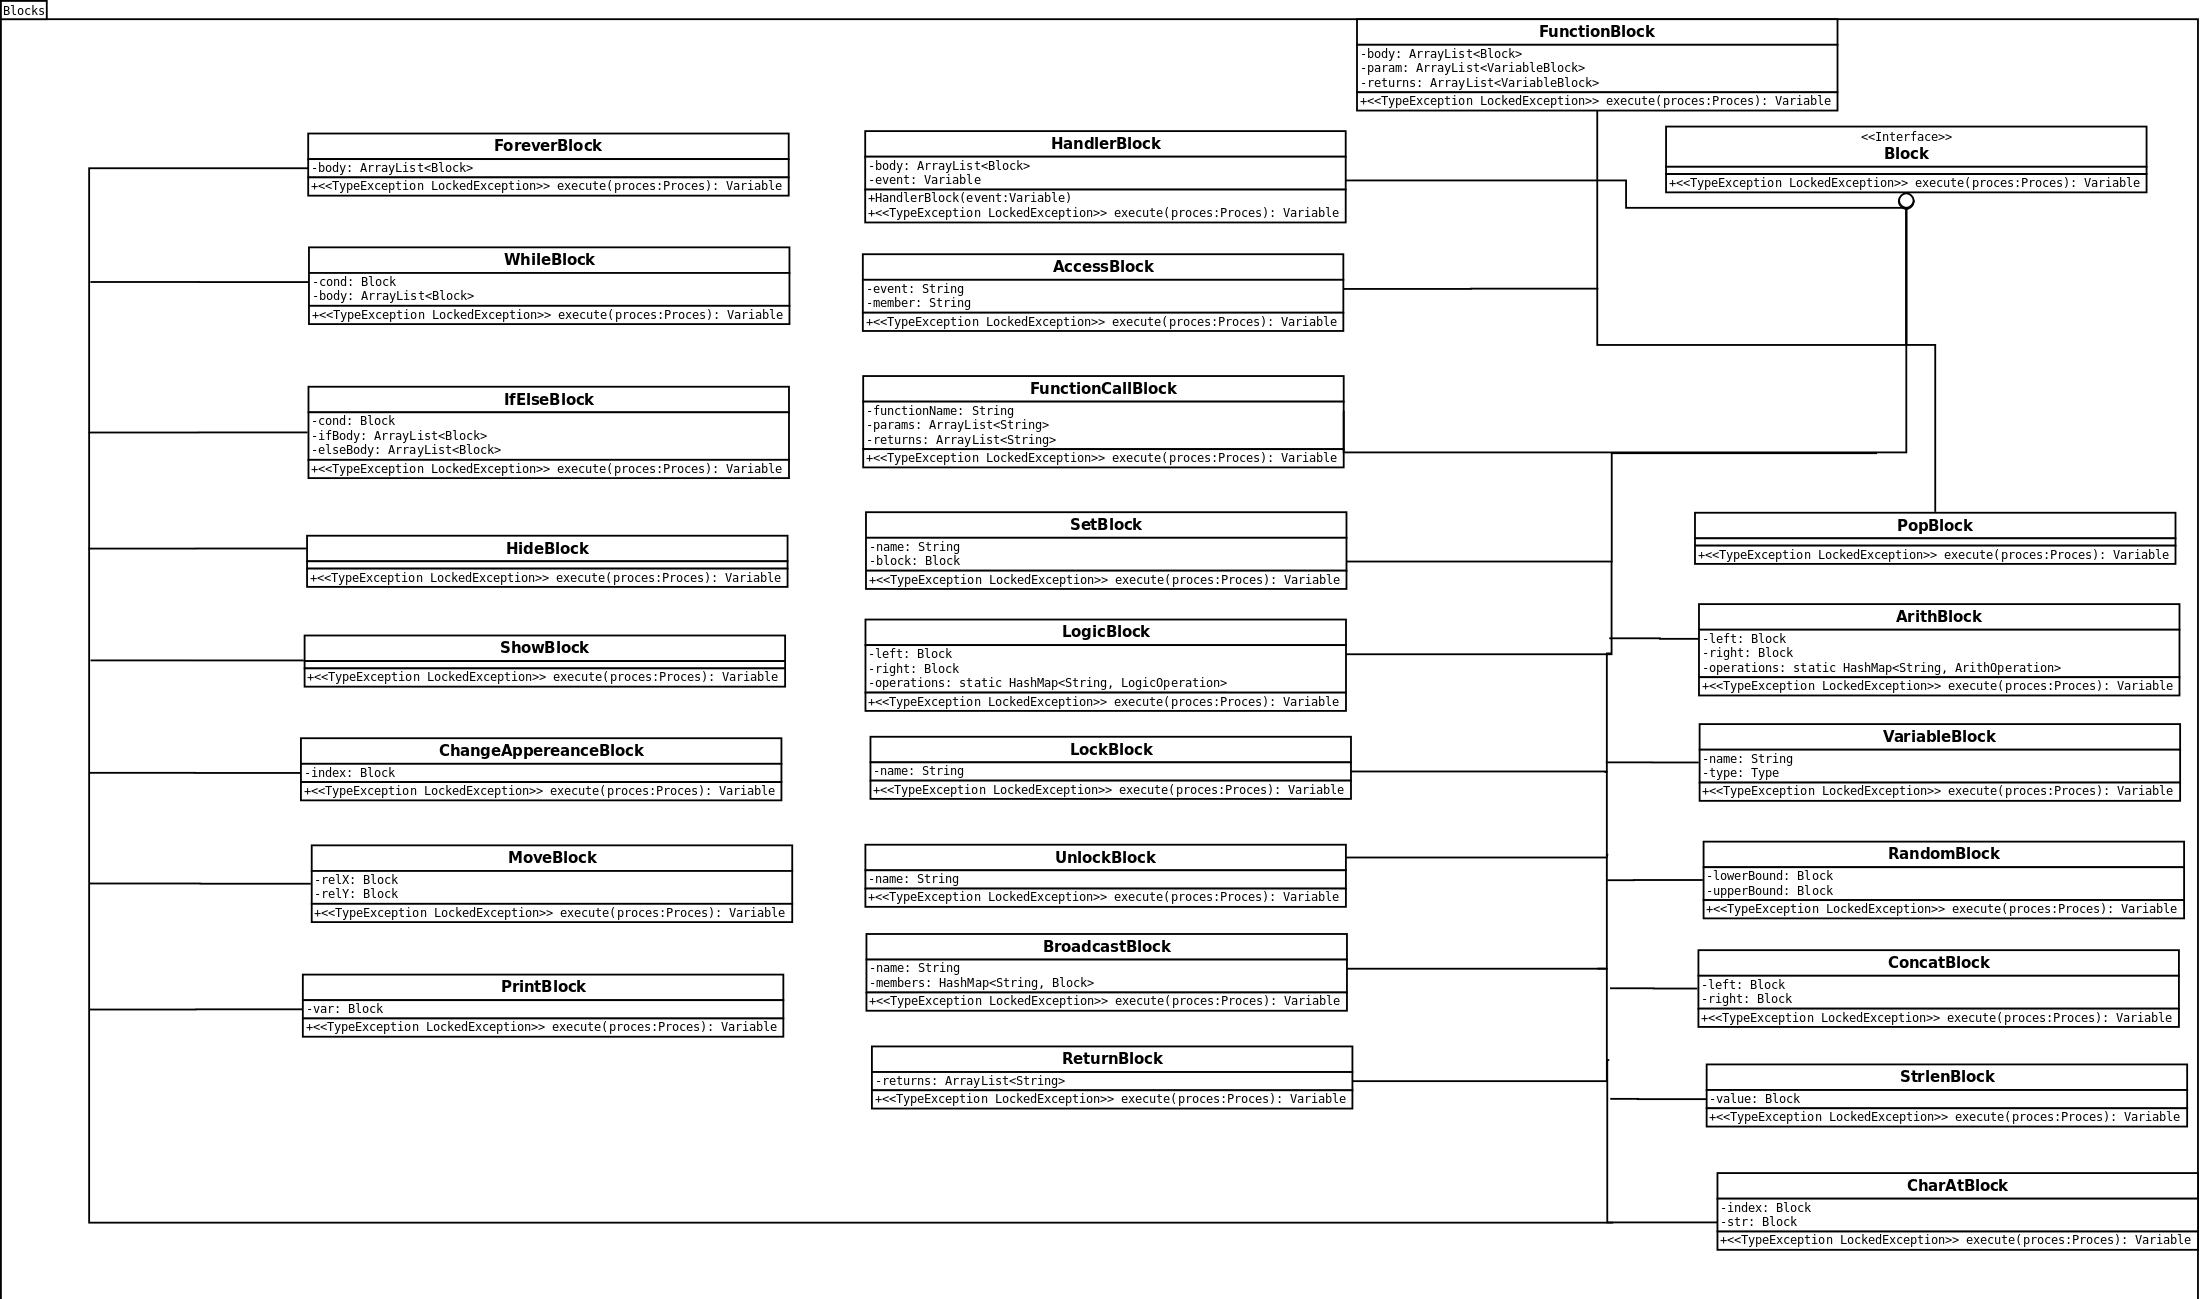
\includegraphics[scale=0.8]{./AnalyseClassenDiagram/block.png}
  \caption{Block Module.} \label{blockUML}
\end{sidewaysfigure}
\clearpage

\subsection{Collections}
De verantwoordelijkheden van deze module worden beschreven in Sectie \ref{CollectionsModule}.
\subsubsection{Classpool}
\label{ClasspoolClass}
Deze bevat alle Classes die aangemaakt zijn in het programma. Deze slaat hij op in een HashMap \cite{hashmap} waarbij een String (de naam) wordt gemapt op een Class. De naam van een Class moet dus uniek zijn.\\\\
\textBF{Keuze ADT's: }
De keuze van een HashMaps \cite{hashmap} zorgt ervoor dat het toevoegen van nieuwe items en het opzoeken van bestaande in O(1) tijd kan gebeuren.
\subsubsection{WiredInstance}
Een wiredInstance bevat een HashMap \cite{hashmap} waarbij een event wordt gemapt op een lijst van instances. We gebruiken hiervoor dus \texttt{java.util.Hashmap<Event, ArrayList<Instance>>} \cite{hashmap} \cite{arraylist}.  Dit stelt alle instances voor die verbonden zijn met \"{e}\"{e}n specifiek uitgaande event van \"{e}\"{e}n specieke instance.
\subsubsection{WireFrame}
\label{WireFrameClass}
Een WireFrame stelt de plaats voorwaarbij alles instanties met elkaar worden verbonden met wires.
Deze bevat een hashmap die Instances mapt op WiredInstances \cite{hashmap}.\\\\
\textBF{Keuze ADT's: }
Door gebruik te maken van deze structuur van Hashmap \cite{hashmap} en WiredInstance kunnen we snel toevoegen en opzoeken. Bij het toevoegen van een wire zal er voor de instance zijn wireFrame worden opgevraagt en voor het event dat verbonden wordt zal de instance waar de wire aankomt worden toegevoegd aan de bijhorende Arraylist \cite{arraylist}. Deze operatie duurt dan O(1) + O(1) + O(1).\\
Het opvragen van alle van instances die verbonden zijn met \'{e}\'{e}n event van \'{e}\'{e}n instance kan dus op dezelfde manier in O(1) + O(1).\\ Het is ons bekend dat het verwijderen van een wire op deze manier niet snel kan verlopen. Het verwijderen gebeurt echter niet op runtime. Daar is het zoeken van belang. We hebben dit in afweging genomen en hebben besloten te gaan voor het snel werken van de VM en dus gekozen voor snel opzoeken.
\subsubsection{EventPool}
\label{EventPoolClass}
Bevat alle Events die in het programma aangemaakt zijn. Deze bewaart hij in een HashMap \cite{hashmap} waarbij een String (het type) wordt gemapt op een Event. Het type van een Event moet dus uniek zijn (voor de hashmap).


\clearpage
 \begin{sidewaysfigure}
  \centering
   
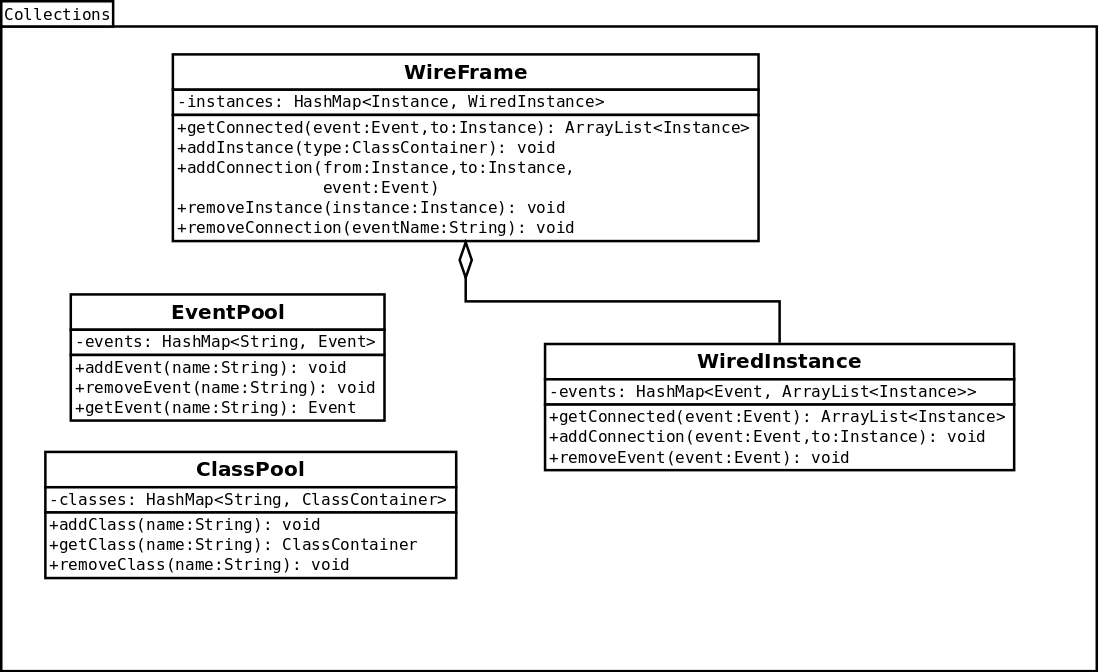
\includegraphics[scale=0.8]{./AnalyseClassenDiagram/collections.png}
  \caption{Collections Module.} \label{collectionsUML}
\end{sidewaysfigure}
\clearpage

\subsection{Core}
De verantwoordelijkheden van deze module worden beschreven in Sectie \ref{CoreModule}.
\subsubsection{Instance}
Deze klasse stelt een instantie van een Class voor. Deze bevat een HashMap \cite{hashmap} van variables deze zijn zijn member variables maar ook zijn positie. Een instance bevat ook zijn Class zodat men weet welke events en functies deze bevat. Een instance bevat ook een HashSet van zijn locked members. 
\subsubsection{EventDispatcher}
\label{eventdispatcher}
De EventDispatcher krijgt een eventInstance en een afzender van de virtual machine. De EventDispatcher kent alle wires en instances. Hij zal voor het gegeven eventInstance alle handlers van de ontvangers opvragen die voor dat event met de afzender zijn verbonden. Voor elke handler cree\"{e}rt hij een nieuw proces dat hij aan de virtual machine geeft.
\subsubsection{Proces}
\label{procesklass}
Het proces bevat een stack van Blocks. Initi\"{e}l bevat die stack enkel de handler die opgeroepen is. Het bevat de instantie waarvan het de handler uitvoert. Het bevat ook een Stack van functionFrames (van Hashmaps waarbij Strings worden gemapt op Variables (zie Sectie \ref{variable})(zie Sectie \ref{functionframe}).\\ Deze laatste stack stelt de stack van actieve functies voor. \\ Een proces bevat een run-functie die \'{e}\'{e}n primitieve stap zal uitvoeren. Deze functie kan een event teruggeven als deze gecree\"{e}rd werd in de primitieve stap. Als het geen event terug geeft is er geen event gecree\"{e}rt maar is het proces nog niet afgelopen. Als het wel een afgelopen (de stack van Blocks is leeg) zal het een ProcesFinishedException gooien. Hierdoor weet de virtualmachine dat het event niet terug op de queue moet worden gezet. Het proces bevat ook nog een klasse ReturnVariables.\\ De klasse bevat ook nog een boolean locked die aangeeft als het proces verantwoordelijk is voor het locken van een variabele. Hierop kunnen er wel nog nieuwe locks gebeuren binnen dat proces. Een voorbeeld van de werking van een proces is uitgewerkt in Sectie \ref{voorbeeldvm}.\\\\
\textBF{Keuze ADT's: }
\label{keuzeHashVar}
De Stack \cite{stack} van Blocks zorgt ervoor dat telkens de bovenste blokken geexecute kunnen worden. De functie wordt er dus telkens volledig bovenop gezet. Omdat we enkel bovenaan moeten toevoegen en uitvoeren gebeurt deze operatie in O(1). We gebruiken hiervoor \texttt{java.util.Stack<Block>} heb Voor informatie over het toevoegen van de blokken van een functie op deze stack verwijzen we naar de Class FunctieBlock.\\\\
Het gebruiken van een Stack \cite{stack} zorgt ervoor dat we weten in welk blok er gezocht moet worden naar de lokale variabele van de huidige functie. Hierdoor kan de totale operatie van zoeken in O(1). Als een variable niet gevonden wordt, zoekt men in de member variables van de instance.
\subsubsection{VirtualMachine}
\label{VMClass}
De virtual machine bevat een lijst (queue) van processen (zie Sectie \ref{procesklass})en de eventDispatcher. Hij doorloopt de lijst van processen door telkens de voorste eraf te halen. Hij zal elk proces \'{e}\'{e}n primitieve stap laten uitvoeren. Als het proces in die primitieve stap een event cree\"{e}rt zal de VM (virtual machine) dit event en zijn zender doorgeven aan de eventDispatcher. Zoals eerder vermeldt zal de eventDispatcher een hoeveelheid processen teruggeven (\texttt{ArrayList<Proces>} \cite{arraylist}). Deze worden achteraan de lijst toegevoegd. Als het huidige proces nog niet is afgerond wordt dit ook achteraan terug toegevoegd (na de eventuele nieuwe processen).\\\\
\textBF{Keuze ADT's: }
Voor de queue gebruiken we \texttt{java.util.LinkedList<Proces>} \cite{linkedlist} hierdoor kan het afnemen van het eerste element en toevoegen van een element aan de queue in O(1). Natuurlijk is de orde van belang in de queue wat hier FIFO is.\\
\subsubsection{FunctionFrame}
\label{functionframe}
Een functionFrame stelt het stackframe voor van een functie blok. Deze bevat een hashmap \cite{hashmap} waarbij
de lokale Variables van die functie gemapt worden op hun naam in die functie.\\\\
\textBF{Keuze ADT's: }
Een Hashmap waarbij Strings worden gemapt op variables. De keuze van een Hashmap zorgt ervoor dat het toevoegen van nieuwe variabelen en het opzoeken van bestaande in O(1) tijd kan gebeuren aangezien een functie een beperkt aantal lokale variabele bevat. Door het gebruik van een Hashmap is er ook geen compile stap nodig omdat we de variable dadelijk kunnen mappen op de content en geen indices van een array moeten worden berekent.\cite{hashmap}
\subsubsection{Event}
Een event bevat een String voor zijn type aan te duiden en een HashMap waarbij het de naam van een variable (String) mapt op een type van variabele. Deze klasse kan een EventInstance van dit event aanmaken \cite{hashmap}.
\subsubsection{Class}
Een Class bevat twee lijsten inputEvents en outputEvents die respecitievelijk alle inkomende en uitgaande events bevatten \cite{arraylist}. Een Hashmap van Strings gemapt op Types die zijn membervariabele voorstellen. De klasse bevat ook twee Hashmaps \cite{hashmap} functions en handlers die respecitievelijk  alle functies en alle handlers bevatten. Bij functions worden functies gemapt op hun naam en bij handlers worden gemapt op het event waarbij ze worden opgeroepen. Een Class is een factory voor zijn instances.

\clearpage
 \begin{sidewaysfigure}
  \centering
   
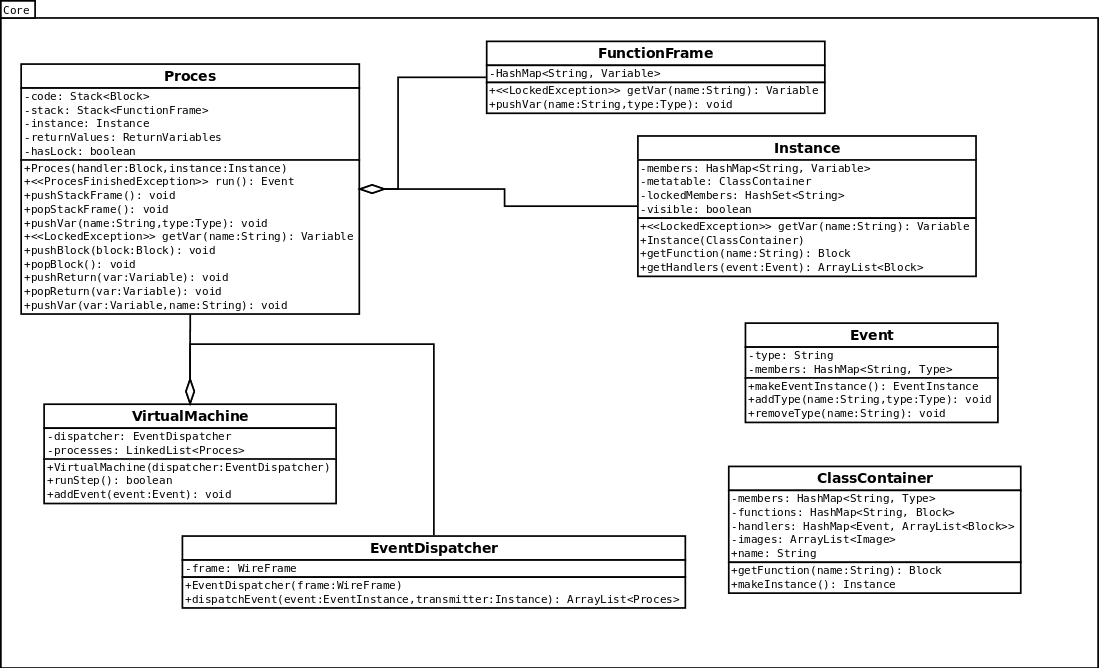
\includegraphics[scale=0.8]{./AnalyseClassenDiagram/core.png}
  \caption{Core Module.} \label{coreUML}
\end{sidewaysfigure}
\clearpage

\subsection{Model}
De verantwoordelijkheden van deze module worden beschreven in Sectie \ref{ModelModule}.
\subsubsection{Abstracte Klasse BlockModel}
\label{ModelBlock}
Deze abstracte klasse wordt als basis voor elk model van bruikbare blokken in de IDE. Deze bevat alle gemeenschappelijke attributen van alle modelen. Deze bestaan uit de positie van het view van die block in de klasse. Alsook een Boolean die aangeeft als de blok moet oplichten bij het debuggen.\\\\ Hieronder geven we enkele afgeleide blokken, een volledige beschrijving zo echter te verleiden voor dit verslag.
\subsubsection{ClassModel}
Deze klasse wordt gebruikt om een klasse in de IDE voor te stellen. Deze bevat de volgende attributen: Alle functieblokken, handlers, naam van de Klasse, outputEvents, member variabelen, images en floatingBlocks. Het gebruik van alle vorige attributen volgt logische uit de beschrijving van een Klasse. Behalve floatingBlocks deze wordt gebruikt voor het groeperen van alle blokken die de gebruiker op het veld van de Klasse heeft geplaats maar nog niet in een functie of handler heeft geplaatst.\\\\
\textBF{Keuze ADT's: }Voor het bijhouden van welk inputEvent wordt afgehandeld door welke handlers gebruiken we een HashMap die het EventModel mapt op een lijst van handlers. Hiervoor gebruiken we \\ \texttt{java.util.Hashmap<EventModel,java.util.ArrayList<HandlerModel>>}. \\ Voor de het bewaren van de member variabele en hun type gebruiken we een Hashmap die de naam van de variabele mapt op een Type \ref{Type}. Hiervoor gebruiken we \texttt{java.util.Hashmap<String, Type>}.
\subsubsection{WhileModel}
Dit is een voorbeeld uitwerking van een BlockModel voor een programmeerblokje. De klasse van een  programmeerblok model die andere blokken kan bevatten heeft voor alle blokken van die klasse een statische lijst van alle BlockModel's die de blok mag bevatten. Aangezien een While-blok twee input velden heeft, scheiden we deze hier door een conditieModel die hier verder wordt uitgewerkt en een lijst van blokken die geaccepteerd zijn in de body.\\\\
\textBF{Keuze ADT's: }
Voor het bijhouden van welke blokken een blok mag bevatten gebruiken we een \texttt{java.util.HashSet<Class>}. Hiermee kan dan worden nagegaan als een blok in een andere kan worden geplaatst. We kiezen voor een HashSet zodat het controlleren een constante tijd kan gebeuren.
\subsubsection{WireFrameModel}
Door dat de compiler de juiste compile functie zoekt op het type, is het WireFrame ook een BlockModel. Deze klasse bevat alle instanties die in het frame staan als ook de wires die ze verbinden. Beide worden bijgehouden in een lijst.
\subsubsection{WireModel}
Dit is een blockModel om een wire voor te stellen. Deze bevat een InstanceModel waarvan het vertrekt en een waar het aankomt. Ook weet de wire welk event het verstuurd.
\subsubsection{InstanceModel}
Dit is een model voor een instance in het WireFrame. Een Instance hoort bij een Klasse. Daarom zal hij de Klasse waarvan hij een instantie is observeren voor veranderingen.

\clearpage
 \begin{sidewaysfigure}
  \centering
   
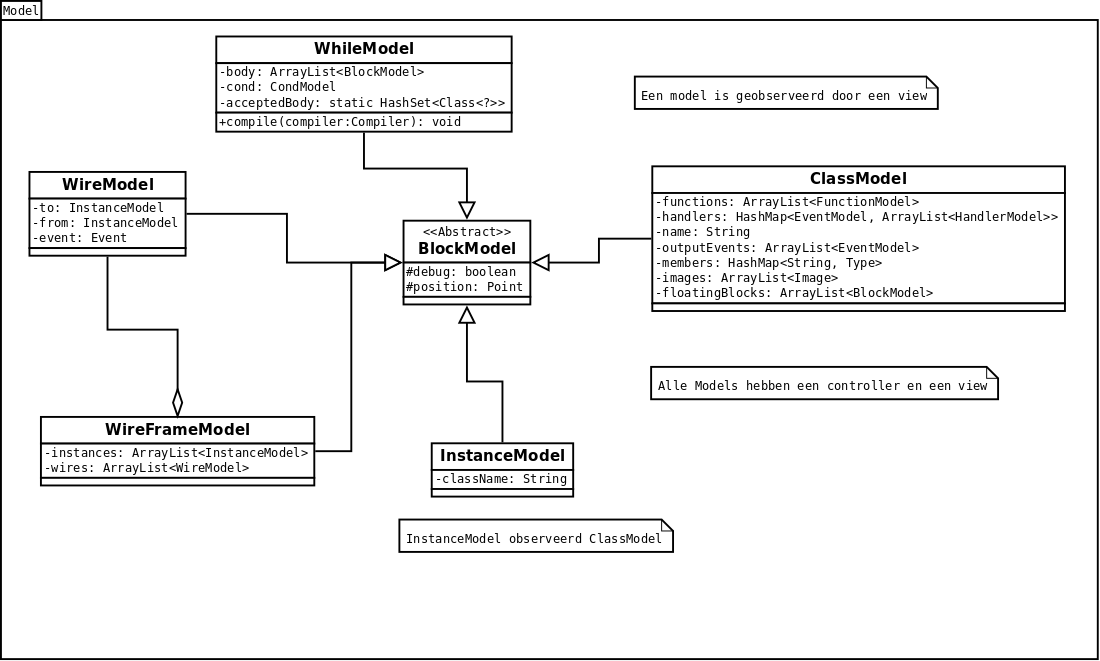
\includegraphics[scale=0.8]{./AnalyseClassenDiagram/model.png}
  \caption{Model Module.} \label{modelUML}
\end{sidewaysfigure}
\clearpage

\subsection{RunTime}
De verantwoordelijkheden van deze module worden beschreven in Sectie \ref{RuntimeModule}.
\subsubsection{Abstracte Klasse Runtime}
Deze klasse wordt gebruikt voor het uitvoeren van het gecree\"{e}rde programma. Alle Klassen en hun blokken zullen eerste door een Compiler die deze klasse bevat gecompileerd worden. Na het succesvol compileren zal de Runtime verantwoordelijk zijn voor het starten van de virtual machine, het stoppen ervan en het doorgeven van inputEvents veroorzaakt door de gebruiker aan deze virtual machine.
\subsubsection{InterpeterRuntime}
\label{runtimeClass}
Dit is de runtime die ge\"{i}mplementeerd zal worden voor dit project. Deze bevat een virtual machine die beschreven wordt in Sectie \ref{VMClass}. De compiler die wordt gebruikt in dit project wordt beschreven in Sectie \ref{IntCompClass}. Deze compiler vult de attributen Classpool, EventPool en WireFrame in deze worden respectievelijk beschreven in Sectie \ref{ClasspoolClass}, Sectie \ref{EventPoolClass} en Sectie \ref{WireFrameClass}.
\subsubsection{Interface Compiler}
We voorzien een Interface voor de compiler zodat er makkelijk een andere compiler kan worden ge\"{i}mplementeerd. Deze bevat een functie voor het compileren van een Runtime.
\subsubsection{InterpeterCompiler}
\label{IntCompClass}
Deze klasse bevat de compiler die ge\"{i}mplementeerd zal worden voor dit project. De bevat functies voor het compileren van een model. Een gedetailleerd beschrijving is te vinden in Sectie \ref{Compileer}.

\clearpage
 \begin{sidewaysfigure}
  \centering
   
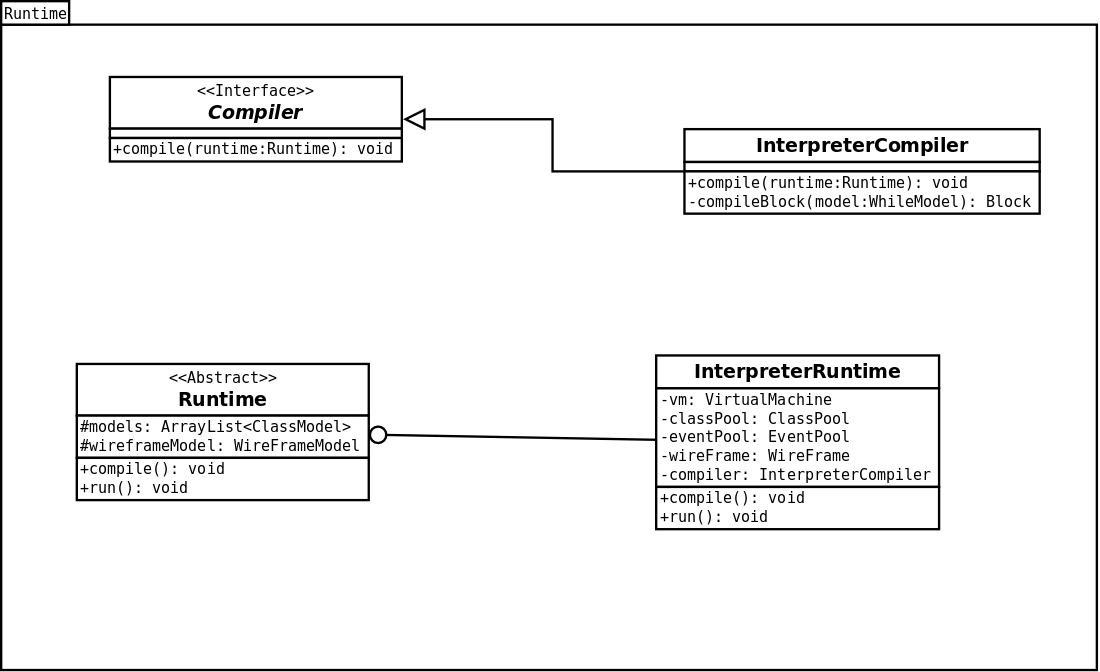
\includegraphics[scale=0.8]{./AnalyseClassenDiagram/runtime.png}
  \caption{Runtime Module.} \label{runtimeUML}
\end{sidewaysfigure}
\clearpage

\subsection{File}
\subsubsection{LanguageModule}
De language class zorgt voor het multilanguage maken van de IDE. Dit gebeurt door een \texttt{ResourceBundle} zoals uitgelegd in Sectie \ref{Multilanguage}

\subsubsection{DataParser}
Een interface klasse die de IDE gebruikt om data te schrijven naar een file. Deze data zal bestaan uit de informatie zijn die nodig is voor projecten die bestaan uit Events, Instanties, Klassen en gerelateerde data.

\subsubsection{XMLParser}
Dit is een implementerende klasse van een DataParser. Deze klasse wordt gebruikt om XML data  te lezen en te schrijven naar een bestand. De XML parser is een information expert met betrekking tot XML data, hij bevat functies waarmee de Modellen van een Klasse, Instantie, enz. geschreven en gelezen kunnen worden. De XML data zelf wordt geparsed door een \texttt{DOMParser} van de Java Standard Library.

\clearpage
 \begin{sidewaysfigure}
  \centering
   
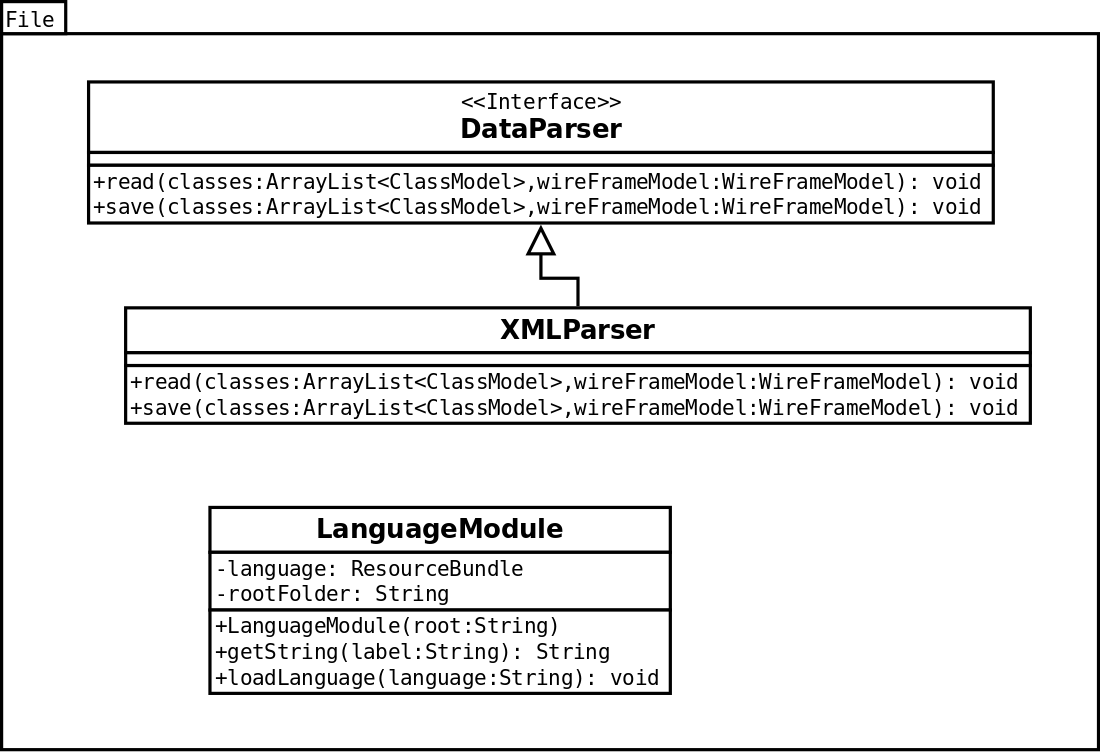
\includegraphics[scale=0.8]{./AnalyseClassenDiagram/file.png}
  \caption{File Module.} \label{file}
\end{sidewaysfigure}
\clearpage


\subsection{GUI}
In dit verslag is enkel de Main klasse uitgewerkt. Dit is de klasse die het JFrame zal bevatten alsook andere noodzakelijke data. Onder andere bevat deze klasse een LanguageModule, een DataParser, een Runtime en Modellen van aangemaakte Klassen/WireFrame

 \begin{figure}[h]
  \centering
   
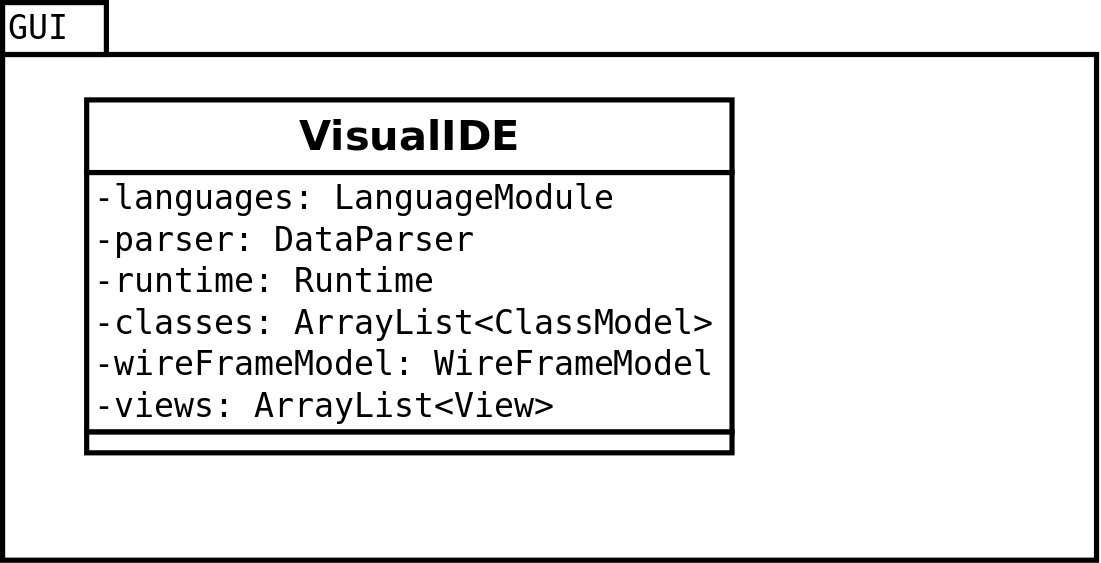
\includegraphics[scale=0.4]{./AnalyseClassenDiagram/gui.png}
  \caption{GUI Module.} \label{gui}
\end{figure}
\clearpage


 
\end{document}